% -----------------------------------------------------------------------------
%                                     HEADER                                    
% -----------------------------------------------------------------------------
\documentclass[a4paper, 10pt]{article}
\usepackage{jheppub}
\usepackage[T1]{fontenc}
\usepackage{colortbl,xcolor,float}
\definecolor{orange}{rgb}{1,0.5,0}
% -----------------------------------------------------------------------------
%                                   COVER PAGE                                  
% -----------------------------------------------------------------------------
\title{{
\includegraphics[scale=.4]{logo.eps}}\ The LaTeX report}

\author{Generated by elijahsheridan on 19 June 2020, 17:44:29}

\abstract{
  This report has been generated automatically
  by {\sc MadAnalysis} 5.\\$~$\\ 
  Please cite:\\ 
  \begin{quote}
    \textbf{E.~Conte, B.~Fuks and G.~Serret},\\ 
    \textit{MadAnalysis 5, A User-Friendly
    Framework for Collider Phenomenology},\\ 
    Comput. Phys. Commun. {\bf 184} (2013) 222-256,\\
    arXiv:1206.1599 [hep-ph].\\ 
  \end{quote}
  To contact us:\\ 
  \begin{quote}
    \textbf{http://madanalysis.irmp.ucl.ac.be}\\
    \textbf{ma5team@iphc.cnrs.fr}\\
  \end{quote}
}

% -----------------------------------------------------------------------------
%                                 BEGIN DOCUMENT                                
% -----------------------------------------------------------------------------
\begin{document}
\maketitle
\flushbottom

% -----------------------------------------------------------------------------
%                                 SECTION Setup                                 
% -----------------------------------------------------------------------------
\newpage
\section{ Setup}

\subsection{ Command history}

\texttt{ma5>\# set directory where running "./\-bin/\-ma5"; set lumi; define the signal significance\\
}
\texttt{ }\texttt{ }\texttt{ma5>set main.currentdir = /\-Users/\-elijahsheridan/\-MG5\_aMC\_v2\_6\_5/\-axion\_pheno/\-madgraph\_data \# need to change this directory path --> exit and type "pwd" to get the path\\
}
\texttt{ }\texttt{ }\texttt{ma5>set main.lumi = 40\\
}
\texttt{ }\texttt{ }\texttt{ma5>set main.fom.formula = 5\\
}
\texttt{ }\texttt{ }\texttt{ma5>set main.fom.x = 0.0\\
}
\texttt{ }\texttt{ }\texttt{ma5>\# import samples --> change the path to the LHE file\\
}
\texttt{ }\texttt{ }\texttt{ma5>import /\-Users/\-elijahsheridan/\-MG5\_aMC\_v2\_6\_5/\-axion\_signal/\-Events/\-1MeV\_gurrola\_cuts\_cross\_sec/\-unweighted\_events.lhe.gz as signal1MeV\\
}
\texttt{ }\texttt{ }\texttt{ma5>import /\-Users/\-elijahsheridan/\-MG5\_aMC\_v2\_6\_5/\-axion\_signal/\-Events/\-100GeV\_gurrola\_cuts\_cross\_sec/\-unweighted\_events.lhe.gz as signal100GeV1TeV\\
}
\texttt{ }\texttt{ }\texttt{ma5>import /\-Users/\-elijahsheridan/\-MG5\_aMC\_v2\_6\_5/\-axion\_signal/\-Events/\-mass100GeV\_Lambda1p5TeV/\-unweighted\_events.lhe.gz as signal100GeV1p5TeV\\
}
\texttt{ }\texttt{ }\texttt{ma5>import /\-Users/\-elijahsheridan/\-MG5\_aMC\_v2\_6\_5/\-axion\_signal/\-Events/\-mass100GeV\_Lambda4TeV/\-unweighted\_events.lhe.gz as signal100GeV4TeV\\
}
\texttt{ }\texttt{ }\texttt{ma5>\# define bg and signal samples\\
}
\texttt{ }\texttt{ }\texttt{ma5>set signal1MeV = signal\\
}
\texttt{ }\texttt{ }\texttt{ma5>set signal100GeV1TeV = signal\\
}
\texttt{ }\texttt{ }\texttt{ma5>set signal100GeV1p5TeV = signal\\
}
\texttt{ }\texttt{ }\texttt{ma5>set signal100GeV4TeV = signal\\
}
\texttt{ }\texttt{ }\texttt{ma5>\# a jet can be from a light quark or b quark\\
}
\texttt{ }\texttt{ }\texttt{ma5>define jets = j\\
}
\texttt{ }\texttt{ }\texttt{ma5>define e = e+ e-\\
}
\texttt{ }\texttt{ }\texttt{ma5>define mu = mu+ mu-\\
}
\texttt{ }\texttt{ }\texttt{ma5>define ta = ta+ ta-\\
}
\texttt{ }\texttt{ }\texttt{ma5>define lept = e mu ta\\
}
\texttt{ }\texttt{ }\texttt{ma5>define ax = 9000005\\
}
\texttt{ }\texttt{ }\texttt{ma5>\# define which plots to make\\
}
\texttt{ }\texttt{ }\texttt{ma5>plot PT(jets[1])\\
}
\texttt{ }\texttt{ }\texttt{ma5>plot ETA(jets[1])\\
}
\texttt{ }\texttt{ }\texttt{ma5>plot PHI(jets[1])\\
}
\texttt{ }\texttt{ }\texttt{ma5>plot PT(jets[2])\\
}
\texttt{ }\texttt{ }\texttt{ma5>plot ETA(jets[2])\\
}
\texttt{ }\texttt{ }\texttt{ma5>plot PHI(jets[2])\\
}
\texttt{ }\texttt{ }\texttt{ma5>plot DELTAR(jets[1], jets[2])\\
}
\texttt{ }\texttt{ }\texttt{ma5>plot M(jets[1] jets[2])\\
}
\texttt{ }\texttt{ }\texttt{ma5>plot sdETA(jets[1] jets[2])\\
}
\texttt{ }\texttt{ }\texttt{ma5>plot THT\\
}
\texttt{ }\texttt{ }\texttt{ma5>plot MET\\
}
\texttt{ }\texttt{ }\texttt{ma5>plot TET\\
}
\texttt{ }\texttt{ }\texttt{ma5>\#set the plot/\-graph parameters\\
}
\texttt{ }\texttt{ }\texttt{ma5>set selection[1].xmin = 0\\
}
\texttt{ }\texttt{ }\texttt{ma5>set selection[1].xmax = 2000\\
}
\texttt{ }\texttt{ }\texttt{ma5>set selection[1].nbins = 200\\
}
\texttt{ }\texttt{ }\texttt{ma5>set selection[1].rank = PTordering\\
}
\texttt{ }\texttt{ }\texttt{ma5>set selection[1].titleX = "p\_\{T\}[j\_\{1\}] (GeV)"\\
}
\texttt{ }\texttt{ }\texttt{ma5>set selection[2].xmin = -8\\
}
\texttt{ }\texttt{ }\texttt{ma5>set selection[2].xmax = 8\\
}
\texttt{ }\texttt{ }\texttt{ma5>set selection[2].nbins = 160\\
}
\texttt{ }\texttt{ }\texttt{ma5>set selection[2].rank = PTordering\\
}
\texttt{ }\texttt{ }\texttt{ma5>set selection[2].titleX = "\#eta[j\_\{1\}]"\\
}
\texttt{ }\texttt{ }\texttt{ma5>set selection[3].xmin = -3.2\\
}
\texttt{ }\texttt{ }\texttt{ma5>set selection[3].xmax = 3.2\\
}
\texttt{ }\texttt{ }\texttt{ma5>set selection[3].nbins = 64\\
}
\texttt{ }\texttt{ }\texttt{ma5>set selection[3].rank = PTordering\\
}
\texttt{ }\texttt{ }\texttt{ma5>set selection[3].titleX = "\#phi[j\_\{1\}]"\\
}
\texttt{ }\texttt{ }\texttt{ma5>set selection[4].xmin = 0\\
}
\texttt{ }\texttt{ }\texttt{ma5>set selection[4].xmax = 1000\\
}
\texttt{ }\texttt{ }\texttt{ma5>set selection[4].nbins = 100\\
}
\texttt{ }\texttt{ }\texttt{ma5>set selection[4].rank = PTordering\\
}
\texttt{ }\texttt{ }\texttt{ma5>set selection[4].titleX = "p\_\{T\}[j\_\{2\}] (GeV)"\\
}
\texttt{ }\texttt{ }\texttt{ma5>set selection[5].xmin = -8\\
}
\texttt{ }\texttt{ }\texttt{ma5>set selection[5].xmax = 8\\
}
\texttt{ }\texttt{ }\texttt{ma5>set selection[5].nbins = 160\\
}
\texttt{ }\texttt{ }\texttt{ma5>set selection[5].rank = PTordering\\
}
\texttt{ }\texttt{ }\texttt{ma5>set selection[5].titleX = "\#eta[j\_\{2\}]"\\
}
\texttt{ }\texttt{ }\texttt{ma5>set selection[6].xmin = -3.2\\
}
\texttt{ }\texttt{ }\texttt{ma5>set selection[6].xmax = 3.2\\
}
\texttt{ }\texttt{ }\texttt{ma5>set selection[6].nbins = 64\\
}
\texttt{ }\texttt{ }\texttt{ma5>set selection[6].rank = PTordering\\
}
\texttt{ }\texttt{ }\texttt{ma5>set selection[6].titleX = "\#phi[j\_\{2\}]"\\
}
\texttt{ }\texttt{ }\texttt{ma5>set selection[7].xmin = 0\\
}
\texttt{ }\texttt{ }\texttt{ma5>set selection[7].xmax = 15\\
}
\texttt{ }\texttt{ }\texttt{ma5>set selection[7].nbins = 75\\
}
\texttt{ }\texttt{ }\texttt{ma5>set selection[7].rank = PTordering\\
}
\texttt{ }\texttt{ }\texttt{ma5>set selection[7].titleX = "\#DeltaR[j\_\{1\},j\_\{2\}]"\\
}
\texttt{ }\texttt{ }\texttt{ma5>set selection[8].xmin = 0\\
}
\texttt{ }\texttt{ }\texttt{ma5>set selection[8].xmax = 3000\\
}
\texttt{ }\texttt{ }\texttt{ma5>set selection[8].nbins = 160\\
}
\texttt{ }\texttt{ }\texttt{ma5>set selection[8].rank = PTordering\\
}
\texttt{ }\texttt{ }\texttt{ma5>set selection[8].titleX = "M[j\_\{1\},j\_\{2\}] (GeV)"\\
}
\texttt{ }\texttt{ }\texttt{ma5>set selection[9].xmin = -15\\
}
\texttt{ }\texttt{ }\texttt{ma5>set selection[9].xmax = 15\\
}
\texttt{ }\texttt{ }\texttt{ma5>set selection[9].titleX = "\#Delta\#eta(j\_\{1\},j\_\{2\})"\\
}
\texttt{ }\texttt{ }\texttt{ma5>set selection[10].xmin = 0\\
}
\texttt{ }\texttt{ }\texttt{ma5>set selection[10].xmax = 4000\\
}
\texttt{ }\texttt{ }\texttt{ma5>set selection[10].nbins = 80\\
}
\texttt{ }\texttt{ }\texttt{ma5>set selection[10].rank = PTordering\\
}
\texttt{ }\texttt{ }\texttt{ma5>set selection[10].titleX = "THT"\\
}
\texttt{ }\texttt{ }\texttt{ma5>set selection[11].xmin = 0\\
}
\texttt{ }\texttt{ }\texttt{ma5>set selection[11].xmax = 1000\\
}
\texttt{ }\texttt{ }\texttt{ma5>set selection[11].nbins = 200\\
}
\texttt{ }\texttt{ }\texttt{ma5>set selection[11].rank = PTordering\\
}
\texttt{ }\texttt{ }\texttt{ma5>set selection[11].titleX = "MET"\\
}
\texttt{ }\texttt{ }\texttt{ma5>set selection[12].xmin = 0\\
}
\texttt{ }\texttt{ }\texttt{ma5>set selection[12].xmax = 8000\\
}
\texttt{ }\texttt{ }\texttt{ma5>set selection[12].nbins = 80\\
}
\texttt{ }\texttt{ }\texttt{ma5>set selection[12].rank = PTordering\\
}
\texttt{ }\texttt{ }\texttt{ma5>set selection[12].titleX = "TET"\\
}
\texttt{ }\texttt{ }\texttt{ma5>submit axion\_masses\_kinematics\_compare\\
}
\texttt{ }\texttt{ }\subsection{ Configuration}

\begin{itemize}
  \item MadAnalysis version 1.6.33 (2017/\-11/\-20).
   \item Histograms given for an integrated luminosity of \textcolor{blue}{40.0}\textcolor{blue}{ fb}$^{\textcolor{blue}{-1}}$\textcolor{blue}{.}
\textcolor{blue}{}
\end{itemize}
% -----------------------------------------------------------------------------
%                                SECTION Datasets                               
% -----------------------------------------------------------------------------
\newpage
\section{ Datasets}

\subsection{ signal1mev}

\begin{itemize}
  \item Sample consisting of: \textcolor{blue}{signal}  events.
   \item Generated events: \textcolor{blue}{1000 }  events.
   \item Normalization to the luminosity: \textcolor{blue}{406568}\textcolor{blue}{ +/\-- }\textcolor{blue}{2950 }  events.
   \item\textcolor{red}{Ratio (event weight): }\textcolor{red}{406 }\textcolor{red}{ - warning: please generate more events (weight larger than 1)!}
\textcolor{red}{}
\end{itemize}
\begin{table}[H]
  \begin{center}
    \begin{tabular}{|m{55.0mm}|m{25.0mm}|m{30.0mm}|m{30.0mm}|}
      \hline
      {\cellcolor{yellow}         Path to the event file}& {\cellcolor{yellow}         Nr. of events}& {\cellcolor{yellow}         Cross section (pb)}& {\cellcolor{yellow}         Negative wgts (\%)}\\
      \hline
      {\cellcolor{white}          axion\_signal/\-Events/\-1MeV\_gurrola\_cuts\_cross\_sec/\-unweighted\_events.lhe.gz}& {\cellcolor{white}          1000}& {\cellcolor{white}          10.2 @ 0.73\%}& {\cellcolor{white}          0.0}\\
\hline
    \end{tabular}
  \end{center}
\end{table}

\subsection{ signal100gev1tev}

\begin{itemize}
  \item Sample consisting of: \textcolor{blue}{signal}  events.
   \item Generated events: \textcolor{blue}{1000 }  events.
   \item Normalization to the luminosity: \textcolor{blue}{340913}\textcolor{blue}{ +/\-- }\textcolor{blue}{3026 }  events.
   \item\textcolor{red}{Ratio (event weight): }\textcolor{red}{340 }\textcolor{red}{ - warning: please generate more events (weight larger than 1)!}
\textcolor{red}{}
\end{itemize}
\begin{table}[H]
  \begin{center}
    \begin{tabular}{|m{55.0mm}|m{25.0mm}|m{30.0mm}|m{30.0mm}|}
      \hline
      {\cellcolor{yellow}         Path to the event file}& {\cellcolor{yellow}         Nr. of events}& {\cellcolor{yellow}         Cross section (pb)}& {\cellcolor{yellow}         Negative wgts (\%)}\\
      \hline
      {\cellcolor{white}          axion\_signal/\-Events/\-100GeV\_gurrola\_cuts\_cross\_sec/\-unweighted\_events.lhe.gz}& {\cellcolor{white}          1000}& {\cellcolor{white}          8.52 @ 0.89\%}& {\cellcolor{white}          0.0}\\
\hline
    \end{tabular}
  \end{center}
\end{table}

\subsection{ signal100gev1p5tev}

\begin{itemize}
  \item Sample consisting of: \textcolor{blue}{signal}  events.
   \item Generated events: \textcolor{blue}{10000 }  events.
   \item Normalization to the luminosity: \textcolor{blue}{71082}\textcolor{blue}{ +/\-- }\textcolor{blue}{222 }  events.
   \item\textcolor{red}{Ratio (event weight): }\textcolor{red}{7.1 }\textcolor{red}{ - warning: please generate more events (weight larger than 1)!}
\textcolor{red}{}
\end{itemize}
\begin{table}[H]
  \begin{center}
    \begin{tabular}{|m{55.0mm}|m{25.0mm}|m{30.0mm}|m{30.0mm}|}
      \hline
      {\cellcolor{yellow}         Path to the event file}& {\cellcolor{yellow}         Nr. of events}& {\cellcolor{yellow}         Cross section (pb)}& {\cellcolor{yellow}         Negative wgts (\%)}\\
      \hline
      {\cellcolor{white}          axion\_signal/\-Events/\-mass100GeV\_Lambda1p5TeV/\-unweighted\_events.lhe.gz}& {\cellcolor{white}          10000}& {\cellcolor{white}          1.78 @ 0.31\%}& {\cellcolor{white}          0.0}\\
\hline
    \end{tabular}
  \end{center}
\end{table}

\subsection{ signal100gev4tev}

\begin{itemize}
  \item Sample consisting of: \textcolor{blue}{signal}  events.
   \item Generated events: \textcolor{blue}{10000 }  events.
   \item Normalization to the luminosity: \textcolor{blue}{7153}\textcolor{blue}{ +/\-- }\textcolor{blue}{20 }  events.
   \item Ratio (event weight): \textcolor{blue}{0.72 } .  
 
\end{itemize}
\begin{table}[H]
  \begin{center}
    \begin{tabular}{|m{55.0mm}|m{25.0mm}|m{30.0mm}|m{30.0mm}|}
      \hline
      {\cellcolor{yellow}         Path to the event file}& {\cellcolor{yellow}         Nr. of events}& {\cellcolor{yellow}         Cross section (pb)}& {\cellcolor{yellow}         Negative wgts (\%)}\\
      \hline
      {\cellcolor{white}          axion\_signal/\-Events/\-mass100GeV\_Lambda4TeV/\-unweighted\_events.lhe.gz}& {\cellcolor{white}          10000}& {\cellcolor{white}          0.179 @ 0.28\%}& {\cellcolor{white}          0.0}\\
\hline
    \end{tabular}
  \end{center}
\end{table}

% -----------------------------------------------------------------------------
%                            SECTION Histos and cuts                            
% -----------------------------------------------------------------------------
\newpage
\section{ Histos and cuts}

\subsection{ Histogram 1}

\textbf{* Plot: PT ( jets[1] ) }\\
   \begin{table}[H]
  \begin{center}
    \begin{tabular}{|m{23.0mm}|m{23.0mm}|m{18.0mm}|m{19.0mm}|m{19.0mm}|m{19.0mm}|m{19.0mm}|}
      \hline
      {\cellcolor{yellow}         Dataset}& {\cellcolor{yellow}         Integral}& {\cellcolor{yellow}         Entries per event}& {\cellcolor{yellow}         Mean}& {\cellcolor{yellow}         RMS}& {\cellcolor{yellow}         \% underflow}& {\cellcolor{yellow}         \% overflow}\\
      \hline
      {\cellcolor{white}         signal1mev}& {\cellcolor{white}         406162}& {\cellcolor{white}         1.0}& {\cellcolor{white}         258.263}& {\cellcolor{white}         210.2}& {\cellcolor{green}         0.0}& {\cellcolor{green}         0.0}\\
      \hline
      {\cellcolor{white}         signal100gev1tev}& {\cellcolor{white}         340572}& {\cellcolor{white}         1.0}& {\cellcolor{white}         314.347}& {\cellcolor{white}         245.4}& {\cellcolor{green}         0.0}& {\cellcolor{green}         0.0}\\
      \hline
      {\cellcolor{white}         signal100gev1p5tev}& {\cellcolor{white}         71075}& {\cellcolor{white}         1.0}& {\cellcolor{white}         241.573}& {\cellcolor{white}         216.5}& {\cellcolor{green}         0.0}& {\cellcolor{green}         0.03}\\
      \hline
      {\cellcolor{white}         signal100gev4tev}& {\cellcolor{white}         7152}& {\cellcolor{white}         1.0}& {\cellcolor{white}         191.202}& {\cellcolor{white}         171.1}& {\cellcolor{green}         0.0}& {\cellcolor{green}         0.0}\\
\hline
    \end{tabular}
  \end{center}
\end{table}

\begin{figure}[H]
  \begin{center}
    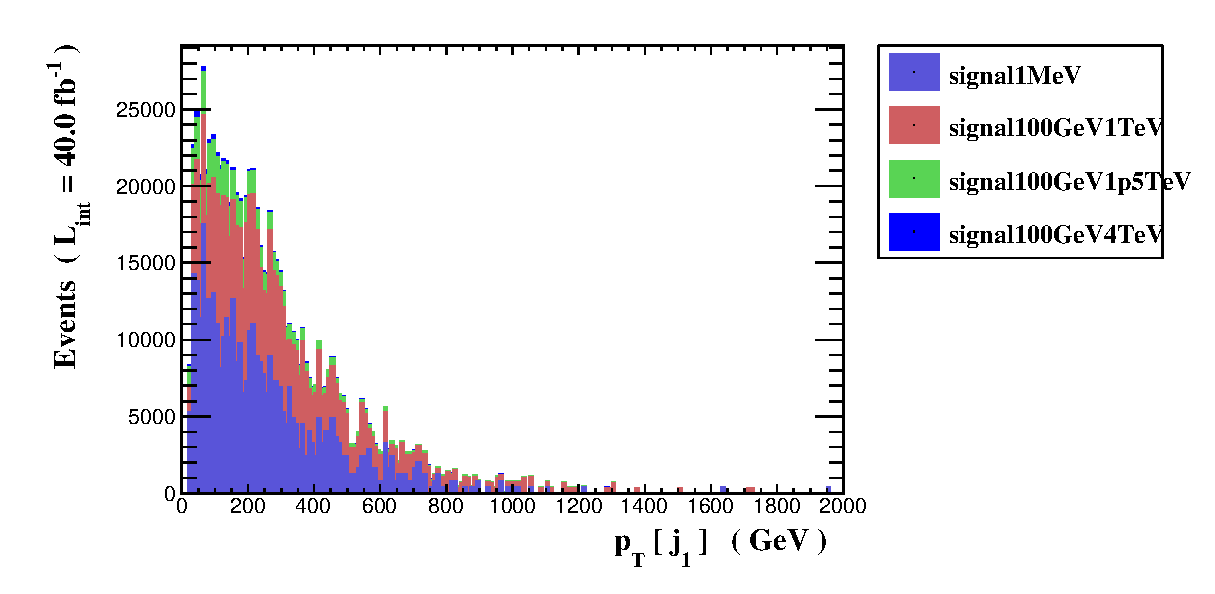
\includegraphics[scale=0.45]{selection_0.eps}\\
\caption{   }
  \end{center}
\end{figure}
      \newpage
\subsection{ Histogram 2}

\textbf{* Plot: ETA ( jets[1] ) }\\
   \begin{table}[H]
  \begin{center}
    \begin{tabular}{|m{23.0mm}|m{23.0mm}|m{18.0mm}|m{19.0mm}|m{19.0mm}|m{19.0mm}|m{19.0mm}|}
      \hline
      {\cellcolor{yellow}         Dataset}& {\cellcolor{yellow}         Integral}& {\cellcolor{yellow}         Entries per event}& {\cellcolor{yellow}         Mean}& {\cellcolor{yellow}         RMS}& {\cellcolor{yellow}         \% underflow}& {\cellcolor{yellow}         \% overflow}\\
      \hline
      {\cellcolor{white}         signal1mev}& {\cellcolor{white}         406162}& {\cellcolor{white}         1.0}& {\cellcolor{white}         0.069541}& {\cellcolor{white}         1.839}& {\cellcolor{green}         0.0}& {\cellcolor{green}         0.0}\\
      \hline
      {\cellcolor{white}         signal100gev1tev}& {\cellcolor{white}         340572}& {\cellcolor{white}         1.0}& {\cellcolor{white}         0.0506079}& {\cellcolor{white}         1.695}& {\cellcolor{green}         0.0}& {\cellcolor{green}         0.0}\\
      \hline
      {\cellcolor{white}         signal100gev1p5tev}& {\cellcolor{white}         71075}& {\cellcolor{white}         1.0}& {\cellcolor{white}         -0.0266127}& {\cellcolor{white}         2.051}& {\cellcolor{green}         0.0}& {\cellcolor{green}         0.0}\\
      \hline
      {\cellcolor{white}         signal100gev4tev}& {\cellcolor{white}         7152}& {\cellcolor{white}         1.0}& {\cellcolor{white}         -0.0218629}& {\cellcolor{white}         2.227}& {\cellcolor{green}         0.0}& {\cellcolor{green}         0.0}\\
\hline
    \end{tabular}
  \end{center}
\end{table}

\begin{figure}[H]
  \begin{center}
    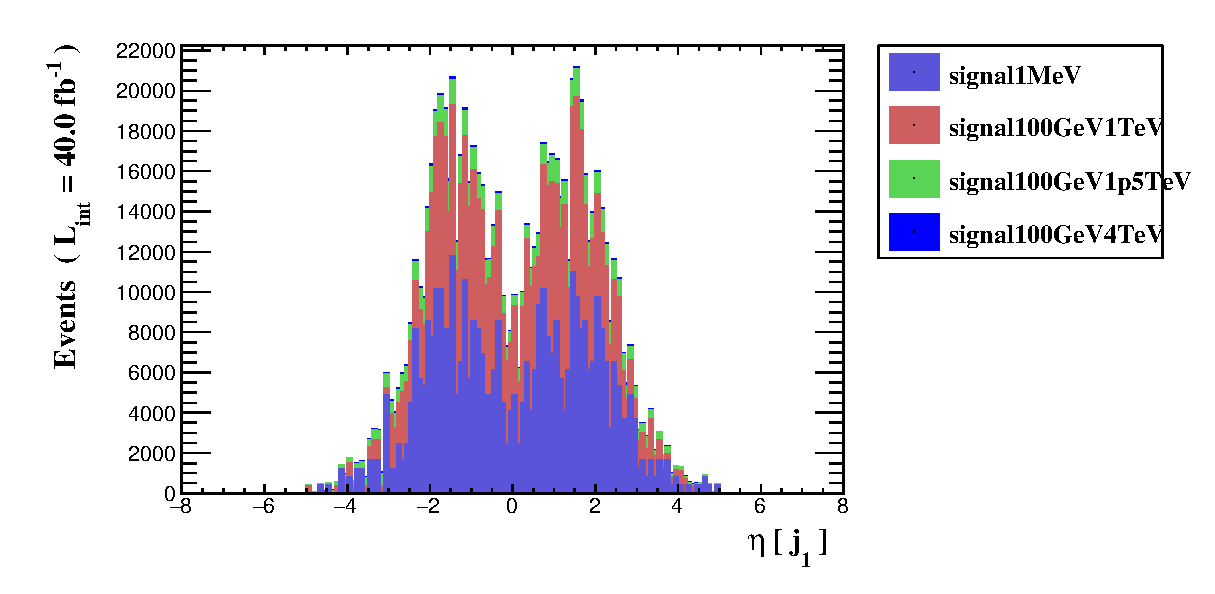
\includegraphics[scale=0.45]{selection_1.eps}\\
\caption{   }
  \end{center}
\end{figure}
      \newpage
\subsection{ Histogram 3}

\textbf{* Plot: PHI ( jets[1] ) }\\
   \begin{table}[H]
  \begin{center}
    \begin{tabular}{|m{23.0mm}|m{23.0mm}|m{18.0mm}|m{19.0mm}|m{19.0mm}|m{19.0mm}|m{19.0mm}|}
      \hline
      {\cellcolor{yellow}         Dataset}& {\cellcolor{yellow}         Integral}& {\cellcolor{yellow}         Entries per event}& {\cellcolor{yellow}         Mean}& {\cellcolor{yellow}         RMS}& {\cellcolor{yellow}         \% underflow}& {\cellcolor{yellow}         \% overflow}\\
      \hline
      {\cellcolor{white}         signal1mev}& {\cellcolor{white}         406162}& {\cellcolor{white}         1.0}& {\cellcolor{white}         0.130532}& {\cellcolor{white}         1.82}& {\cellcolor{green}         0.0}& {\cellcolor{green}         0.0}\\
      \hline
      {\cellcolor{white}         signal100gev1tev}& {\cellcolor{white}         340572}& {\cellcolor{white}         1.0}& {\cellcolor{white}         0.0367644}& {\cellcolor{white}         1.84}& {\cellcolor{green}         0.0}& {\cellcolor{green}         0.0}\\
      \hline
      {\cellcolor{white}         signal100gev1p5tev}& {\cellcolor{white}         71075}& {\cellcolor{white}         1.0}& {\cellcolor{white}         -0.0191116}& {\cellcolor{white}         1.806}& {\cellcolor{green}         0.0}& {\cellcolor{green}         0.0}\\
      \hline
      {\cellcolor{white}         signal100gev4tev}& {\cellcolor{white}         7152}& {\cellcolor{white}         1.0}& {\cellcolor{white}         0.0265117}& {\cellcolor{white}         1.818}& {\cellcolor{green}         0.0}& {\cellcolor{green}         0.0}\\
\hline
    \end{tabular}
  \end{center}
\end{table}

\begin{figure}[H]
  \begin{center}
    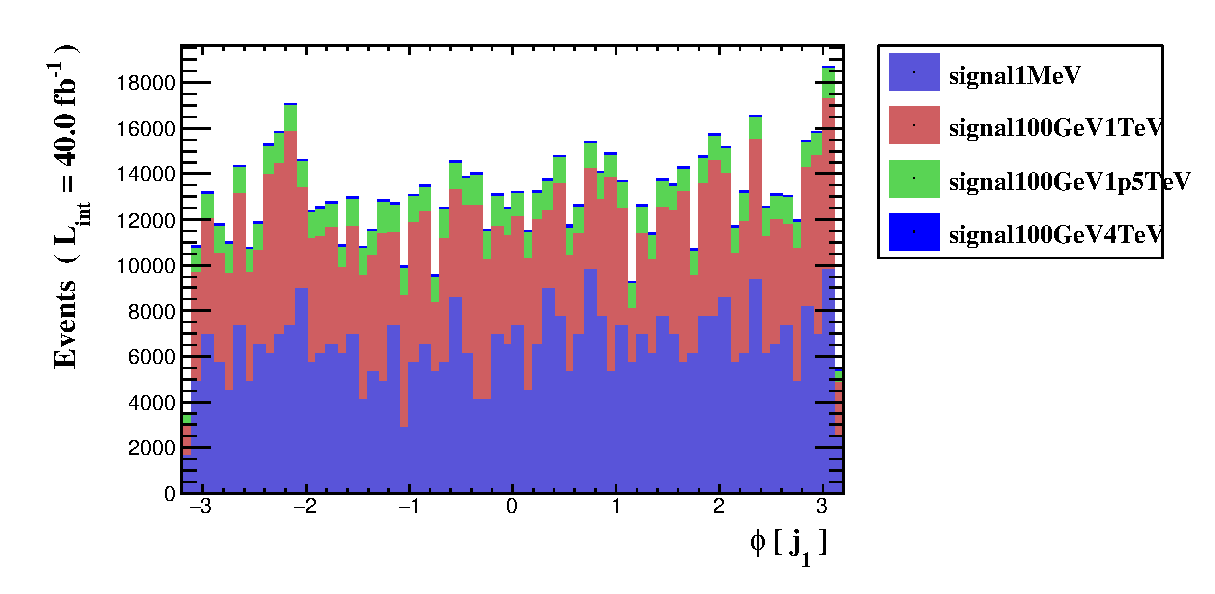
\includegraphics[scale=0.45]{selection_2.eps}\\
\caption{   }
  \end{center}
\end{figure}
      \newpage
\subsection{ Histogram 4}

\textbf{* Plot: PT ( jets[2] ) }\\
   \begin{table}[H]
  \begin{center}
    \begin{tabular}{|m{23.0mm}|m{23.0mm}|m{18.0mm}|m{19.0mm}|m{19.0mm}|m{19.0mm}|m{19.0mm}|}
      \hline
      {\cellcolor{yellow}         Dataset}& {\cellcolor{yellow}         Integral}& {\cellcolor{yellow}         Entries per event}& {\cellcolor{yellow}         Mean}& {\cellcolor{yellow}         RMS}& {\cellcolor{yellow}         \% underflow}& {\cellcolor{yellow}         \% overflow}\\
      \hline
      {\cellcolor{white}         signal1mev}& {\cellcolor{white}         406162}& {\cellcolor{white}         1.0}& {\cellcolor{white}         121.574}& {\cellcolor{white}         112.1}& {\cellcolor{green}         0.0}& {\cellcolor{green}         0.0}\\
      \hline
      {\cellcolor{white}         signal100gev1tev}& {\cellcolor{white}         340572}& {\cellcolor{white}         1.0}& {\cellcolor{white}         136.673}& {\cellcolor{white}         117.6}& {\cellcolor{green}         0.0}& {\cellcolor{green}         0.0}\\
      \hline
      {\cellcolor{white}         signal100gev1p5tev}& {\cellcolor{white}         71075}& {\cellcolor{white}         1.0}& {\cellcolor{white}         102.544}& {\cellcolor{white}         100.5}& {\cellcolor{green}         0.0}& {\cellcolor{green}         0.04}\\
      \hline
      {\cellcolor{white}         signal100gev4tev}& {\cellcolor{white}         7152}& {\cellcolor{white}         1.0}& {\cellcolor{white}         78.381}& {\cellcolor{white}         70.87}& {\cellcolor{green}         0.0}& {\cellcolor{green}         0.01}\\
\hline
    \end{tabular}
  \end{center}
\end{table}

\begin{figure}[H]
  \begin{center}
    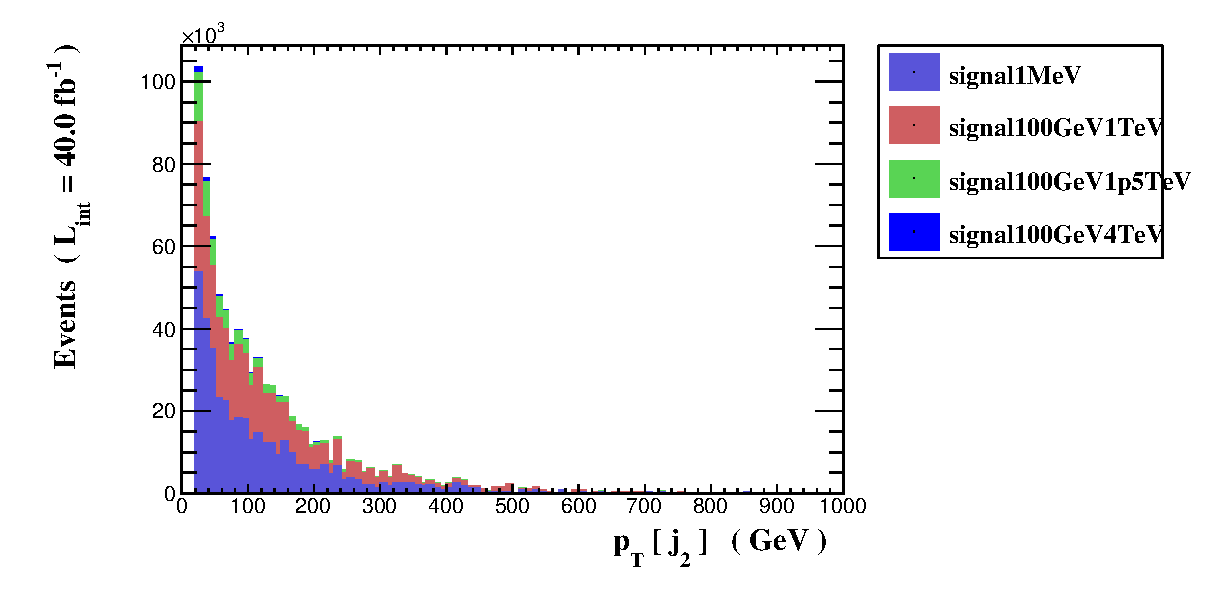
\includegraphics[scale=0.45]{selection_3.eps}\\
\caption{   }
  \end{center}
\end{figure}
      \newpage
\subsection{ Histogram 5}

\textbf{* Plot: ETA ( jets[2] ) }\\
   \begin{table}[H]
  \begin{center}
    \begin{tabular}{|m{23.0mm}|m{23.0mm}|m{18.0mm}|m{19.0mm}|m{19.0mm}|m{19.0mm}|m{19.0mm}|}
      \hline
      {\cellcolor{yellow}         Dataset}& {\cellcolor{yellow}         Integral}& {\cellcolor{yellow}         Entries per event}& {\cellcolor{yellow}         Mean}& {\cellcolor{yellow}         RMS}& {\cellcolor{yellow}         \% underflow}& {\cellcolor{yellow}         \% overflow}\\
      \hline
      {\cellcolor{white}         signal1mev}& {\cellcolor{white}         406162}& {\cellcolor{white}         1.0}& {\cellcolor{white}         -0.0527262}& {\cellcolor{white}         2.281}& {\cellcolor{green}         0.0}& {\cellcolor{green}         0.0}\\
      \hline
      {\cellcolor{white}         signal100gev1tev}& {\cellcolor{white}         340572}& {\cellcolor{white}         1.0}& {\cellcolor{white}         -0.00108636}& {\cellcolor{white}         2.3}& {\cellcolor{green}         0.0}& {\cellcolor{green}         0.0}\\
      \hline
      {\cellcolor{white}         signal100gev1p5tev}& {\cellcolor{white}         71075}& {\cellcolor{white}         1.0}& {\cellcolor{white}         0.0588376}& {\cellcolor{white}         2.589}& {\cellcolor{green}         0.0}& {\cellcolor{green}         0.0}\\
      \hline
      {\cellcolor{white}         signal100gev4tev}& {\cellcolor{white}         7152}& {\cellcolor{white}         1.0}& {\cellcolor{white}         0.00814923}& {\cellcolor{white}         2.789}& {\cellcolor{green}         0.0}& {\cellcolor{green}         0.0}\\
\hline
    \end{tabular}
  \end{center}
\end{table}

\begin{figure}[H]
  \begin{center}
    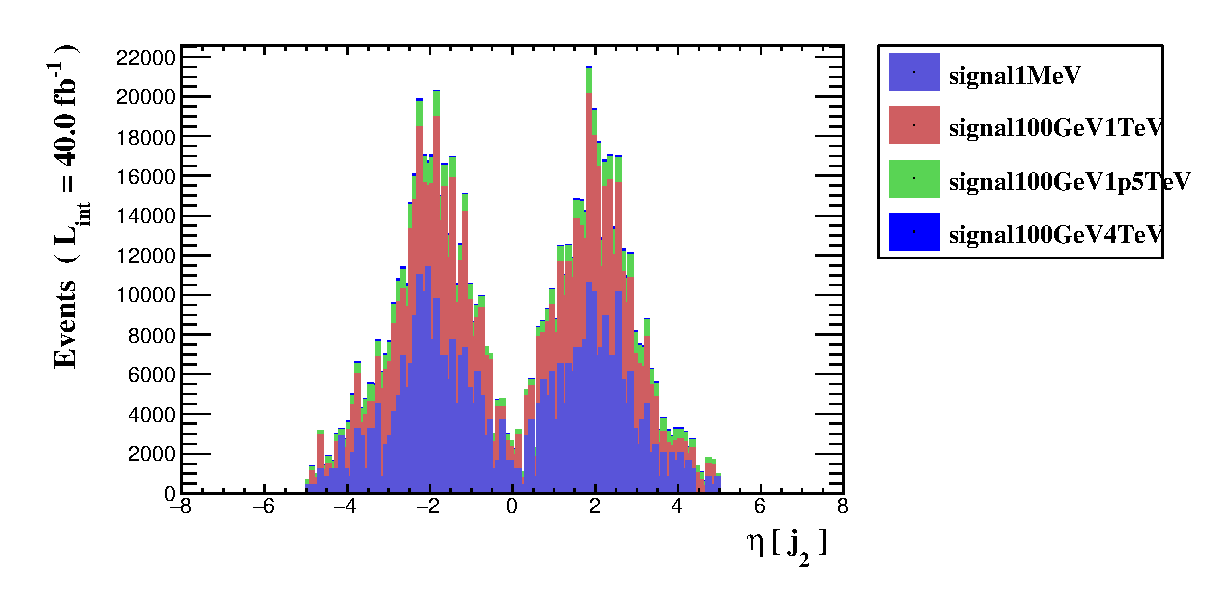
\includegraphics[scale=0.45]{selection_4.eps}\\
\caption{   }
  \end{center}
\end{figure}
      \newpage
\subsection{ Histogram 6}

\textbf{* Plot: PHI ( jets[2] ) }\\
   \begin{table}[H]
  \begin{center}
    \begin{tabular}{|m{23.0mm}|m{23.0mm}|m{18.0mm}|m{19.0mm}|m{19.0mm}|m{19.0mm}|m{19.0mm}|}
      \hline
      {\cellcolor{yellow}         Dataset}& {\cellcolor{yellow}         Integral}& {\cellcolor{yellow}         Entries per event}& {\cellcolor{yellow}         Mean}& {\cellcolor{yellow}         RMS}& {\cellcolor{yellow}         \% underflow}& {\cellcolor{yellow}         \% overflow}\\
      \hline
      {\cellcolor{white}         signal1mev}& {\cellcolor{white}         406162}& {\cellcolor{white}         1.0}& {\cellcolor{white}         0.0258354}& {\cellcolor{white}         1.803}& {\cellcolor{green}         0.0}& {\cellcolor{green}         0.0}\\
      \hline
      {\cellcolor{white}         signal100gev1tev}& {\cellcolor{white}         340572}& {\cellcolor{white}         1.0}& {\cellcolor{white}         0.0083797}& {\cellcolor{white}         1.807}& {\cellcolor{green}         0.0}& {\cellcolor{green}         0.0}\\
      \hline
      {\cellcolor{white}         signal100gev1p5tev}& {\cellcolor{white}         71075}& {\cellcolor{white}         1.0}& {\cellcolor{white}         -0.0105592}& {\cellcolor{white}         1.815}& {\cellcolor{green}         0.0}& {\cellcolor{green}         0.0}\\
      \hline
      {\cellcolor{white}         signal100gev4tev}& {\cellcolor{white}         7152}& {\cellcolor{white}         1.0}& {\cellcolor{white}         -0.000478749}& {\cellcolor{white}         1.832}& {\cellcolor{green}         0.0}& {\cellcolor{green}         0.0}\\
\hline
    \end{tabular}
  \end{center}
\end{table}

\begin{figure}[H]
  \begin{center}
    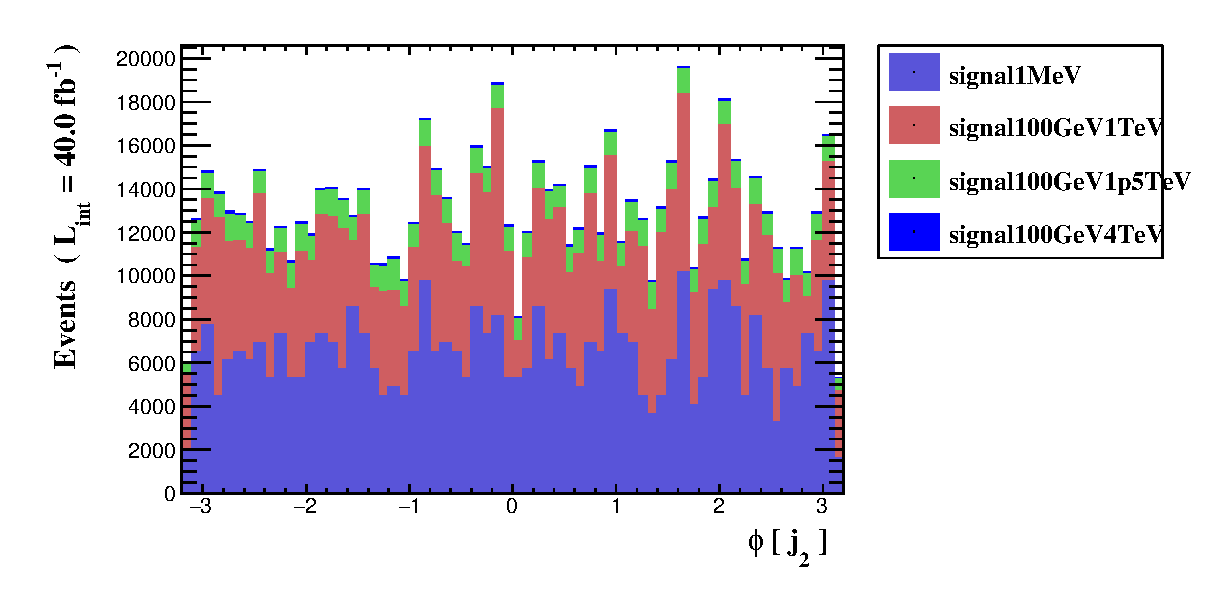
\includegraphics[scale=0.45]{selection_5.eps}\\
\caption{   }
  \end{center}
\end{figure}
      \newpage
\subsection{ Histogram 7}

\textbf{* Plot: DELTAR ( jets[1] , jets[2] ) }\\
   \begin{table}[H]
  \begin{center}
    \begin{tabular}{|m{23.0mm}|m{23.0mm}|m{18.0mm}|m{19.0mm}|m{19.0mm}|m{19.0mm}|m{19.0mm}|}
      \hline
      {\cellcolor{yellow}         Dataset}& {\cellcolor{yellow}         Integral}& {\cellcolor{yellow}         Entries per event}& {\cellcolor{yellow}         Mean}& {\cellcolor{yellow}         RMS}& {\cellcolor{yellow}         \% underflow}& {\cellcolor{yellow}         \% overflow}\\
      \hline
      {\cellcolor{white}         signal1mev}& {\cellcolor{white}         406162}& {\cellcolor{white}         1.0}& {\cellcolor{white}         4.21235}& {\cellcolor{white}         1.039}& {\cellcolor{green}         0.0}& {\cellcolor{green}         0.0}\\
      \hline
      {\cellcolor{white}         signal100gev1tev}& {\cellcolor{white}         340572}& {\cellcolor{white}         1.0}& {\cellcolor{white}         4.08377}& {\cellcolor{white}         1.031}& {\cellcolor{green}         0.0}& {\cellcolor{green}         0.0}\\
      \hline
      {\cellcolor{white}         signal100gev1p5tev}& {\cellcolor{white}         71075}& {\cellcolor{white}         1.0}& {\cellcolor{white}         4.55035}& {\cellcolor{white}         1.26}& {\cellcolor{green}         0.0}& {\cellcolor{green}         0.0}\\
      \hline
      {\cellcolor{white}         signal100gev4tev}& {\cellcolor{white}         7152}& {\cellcolor{white}         1.0}& {\cellcolor{white}         4.85618}& {\cellcolor{white}         1.299}& {\cellcolor{green}         0.0}& {\cellcolor{green}         0.0}\\
\hline
    \end{tabular}
  \end{center}
\end{table}

\begin{figure}[H]
  \begin{center}
    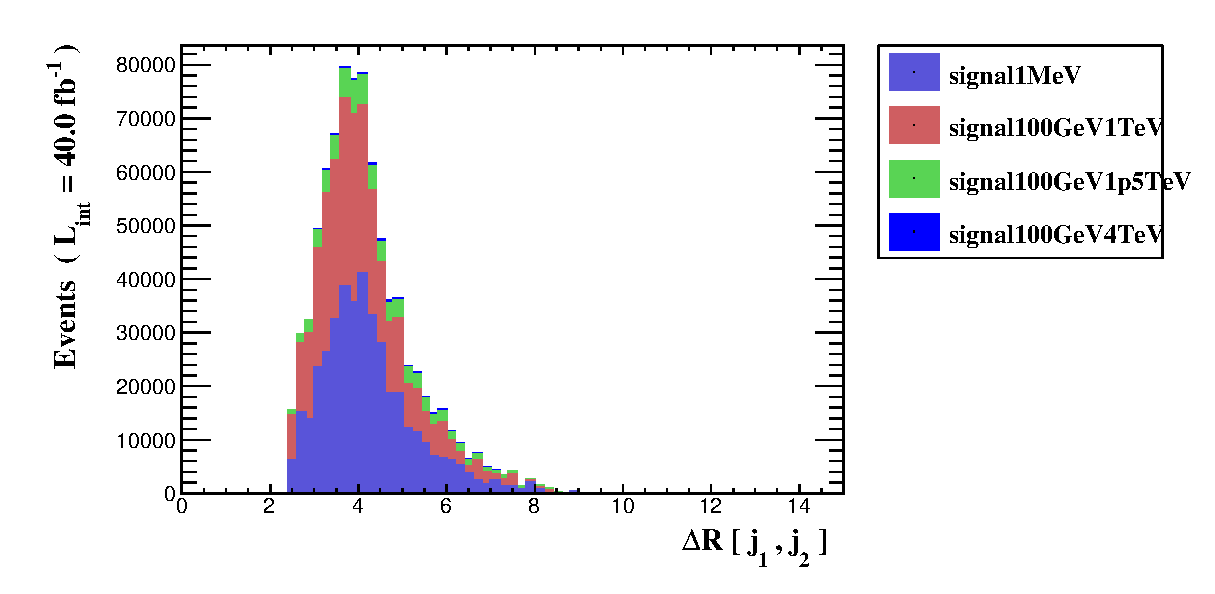
\includegraphics[scale=0.45]{selection_6.eps}\\
\caption{   }
  \end{center}
\end{figure}
      \newpage
\subsection{ Histogram 8}

\textbf{* Plot: M ( jets[1] jets[2] ) }\\
   \begin{table}[H]
  \begin{center}
    \begin{tabular}{|m{23.0mm}|m{23.0mm}|m{18.0mm}|m{19.0mm}|m{19.0mm}|m{19.0mm}|m{19.0mm}|}
      \hline
      {\cellcolor{yellow}         Dataset}& {\cellcolor{yellow}         Integral}& {\cellcolor{yellow}         Entries per event}& {\cellcolor{yellow}         Mean}& {\cellcolor{yellow}         RMS}& {\cellcolor{yellow}         \% underflow}& {\cellcolor{yellow}         \% overflow}\\
      \hline
      {\cellcolor{white}         signal1mev}& {\cellcolor{white}         406162}& {\cellcolor{white}         1.0}& {\cellcolor{white}         985.186}& {\cellcolor{white}         666.7}& {\cellcolor{green}         0.0}& {\cellcolor{green}         1.602}\\
      \hline
      {\cellcolor{white}         signal100gev1tev}& {\cellcolor{white}         340572}& {\cellcolor{white}         1.0}& {\cellcolor{white}         1094.3}& {\cellcolor{white}         687.1}& {\cellcolor{green}         0.0}& {\cellcolor{green}         2.202}\\
      \hline
      {\cellcolor{white}         signal100gev1p5tev}& {\cellcolor{white}         71075}& {\cellcolor{white}         1.0}& {\cellcolor{white}         1110.02}& {\cellcolor{white}         786.2}& {\cellcolor{green}         0.0}& {\cellcolor{green}         3.11}\\
      \hline
      {\cellcolor{white}         signal100gev4tev}& {\cellcolor{white}         7152}& {\cellcolor{white}         1.0}& {\cellcolor{white}         1096.34}& {\cellcolor{white}         808.0}& {\cellcolor{green}         0.0}& {\cellcolor{green}         3.8}\\
\hline
    \end{tabular}
  \end{center}
\end{table}

\begin{figure}[H]
  \begin{center}
    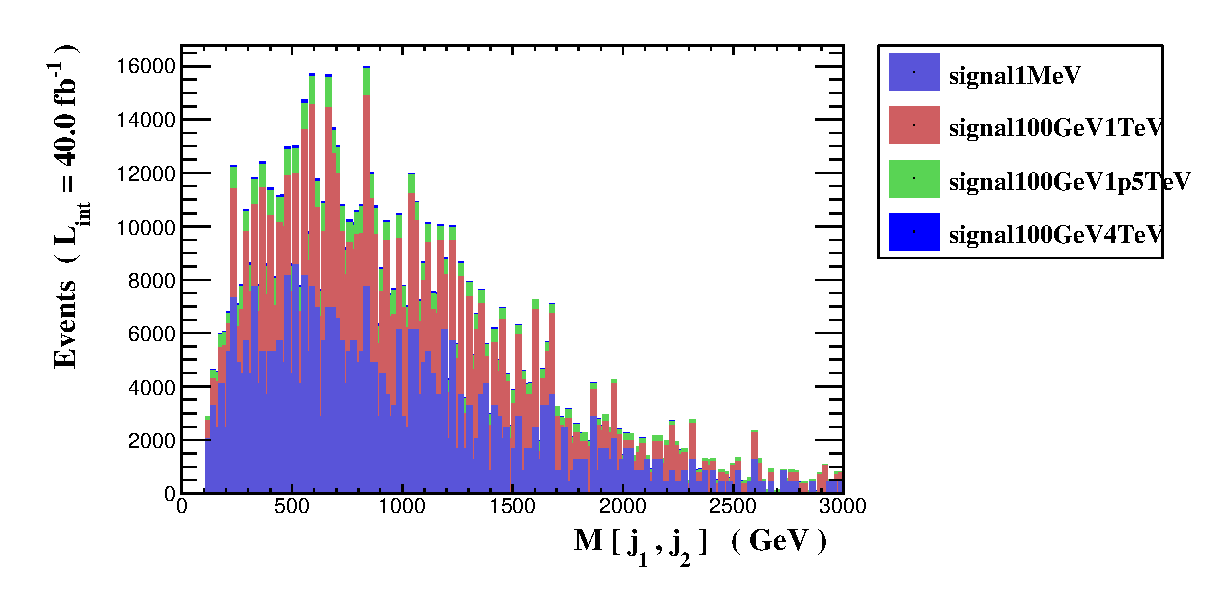
\includegraphics[scale=0.45]{selection_7.eps}\\
\caption{   }
  \end{center}
\end{figure}
      \newpage
\subsection{ Histogram 9}

\textbf{* Plot: sdETA ( jets[1] jets[2] ) }\\
   \begin{table}[H]
  \begin{center}
    \begin{tabular}{|m{23.0mm}|m{23.0mm}|m{18.0mm}|m{19.0mm}|m{19.0mm}|m{19.0mm}|m{19.0mm}|}
      \hline
      {\cellcolor{yellow}         Dataset}& {\cellcolor{yellow}         Integral}& {\cellcolor{yellow}         Entries per event}& {\cellcolor{yellow}         Mean}& {\cellcolor{yellow}         RMS}& {\cellcolor{yellow}         \% underflow}& {\cellcolor{yellow}         \% overflow}\\
      \hline
      {\cellcolor{white}         signal1mev}& {\cellcolor{white}         406162}& {\cellcolor{white}         1.0}& {\cellcolor{white}         0.122267}& {\cellcolor{white}         3.815}& {\cellcolor{green}         0.0}& {\cellcolor{green}         0.0}\\
      \hline
      {\cellcolor{white}         signal100gev1tev}& {\cellcolor{white}         340572}& {\cellcolor{white}         1.0}& {\cellcolor{white}         0.0516943}& {\cellcolor{white}         3.713}& {\cellcolor{green}         0.0}& {\cellcolor{green}         0.0}\\
      \hline
      {\cellcolor{white}         signal100gev1p5tev}& {\cellcolor{white}         71075}& {\cellcolor{white}         1.0}& {\cellcolor{white}         -0.0854503}& {\cellcolor{white}         4.338}& {\cellcolor{green}         0.0}& {\cellcolor{green}         0.0}\\
      \hline
      {\cellcolor{white}         signal100gev4tev}& {\cellcolor{white}         7152}& {\cellcolor{white}         1.0}& {\cellcolor{white}         -0.0300121}& {\cellcolor{white}         4.701}& {\cellcolor{green}         0.0}& {\cellcolor{green}         0.0}\\
\hline
    \end{tabular}
  \end{center}
\end{table}

\begin{figure}[H]
  \begin{center}
    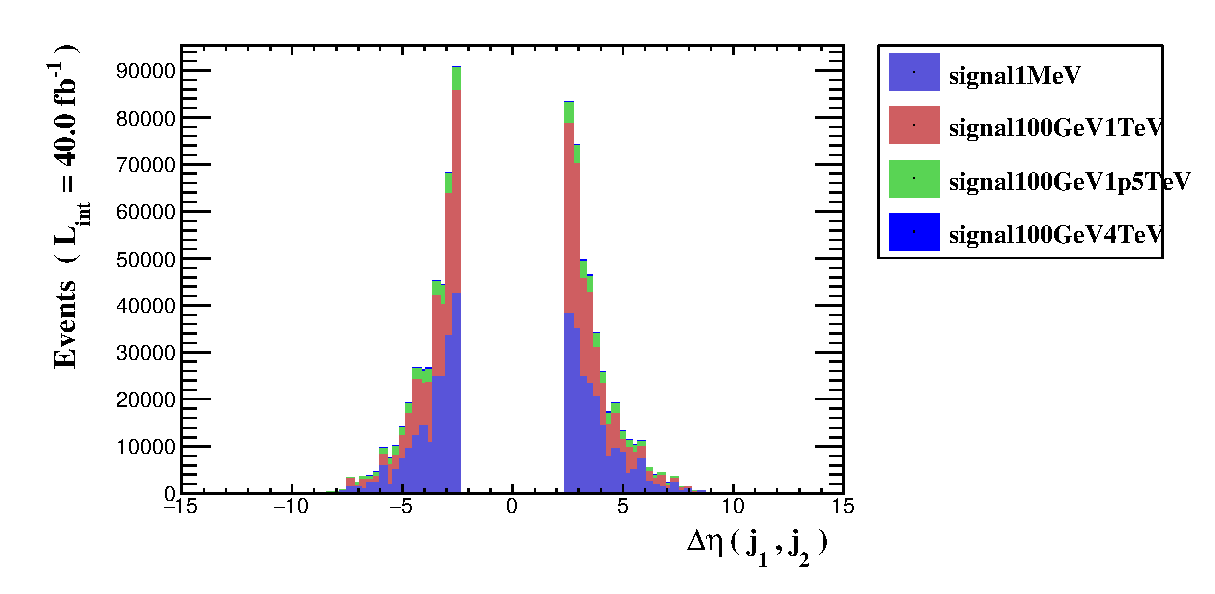
\includegraphics[scale=0.45]{selection_8.eps}\\
\caption{   }
  \end{center}
\end{figure}
      \newpage
\subsection{ Histogram 10}

\textbf{* Plot: THT}\\
   \begin{table}[H]
  \begin{center}
    \begin{tabular}{|m{23.0mm}|m{23.0mm}|m{18.0mm}|m{19.0mm}|m{19.0mm}|m{19.0mm}|m{19.0mm}|}
      \hline
      {\cellcolor{yellow}         Dataset}& {\cellcolor{yellow}         Integral}& {\cellcolor{yellow}         Entries per event}& {\cellcolor{yellow}         Mean}& {\cellcolor{yellow}         RMS}& {\cellcolor{yellow}         \% underflow}& {\cellcolor{yellow}         \% overflow}\\
      \hline
      {\cellcolor{white}         signal1mev}& {\cellcolor{white}         406568}& {\cellcolor{white}         1.0}& {\cellcolor{white}         379.799}& {\cellcolor{white}         289.9}& {\cellcolor{green}         0.0}& {\cellcolor{green}         0.0}\\
      \hline
      {\cellcolor{white}         signal100gev1tev}& {\cellcolor{white}         340913}& {\cellcolor{white}         1.0}& {\cellcolor{white}         450.967}& {\cellcolor{white}         323.8}& {\cellcolor{green}         0.0}& {\cellcolor{green}         0.0}\\
      \hline
      {\cellcolor{white}         signal100gev1p5tev}& {\cellcolor{white}         71082}& {\cellcolor{white}         1.0}& {\cellcolor{white}         344.097}& {\cellcolor{white}         286.7}& {\cellcolor{green}         0.0}& {\cellcolor{green}         0.0}\\
      \hline
      {\cellcolor{white}         signal100gev4tev}& {\cellcolor{white}         7153}& {\cellcolor{white}         1.0}& {\cellcolor{white}         269.432}& {\cellcolor{white}         217.8}& {\cellcolor{green}         0.0}& {\cellcolor{green}         0.0}\\
\hline
    \end{tabular}
  \end{center}
\end{table}

\begin{figure}[H]
  \begin{center}
    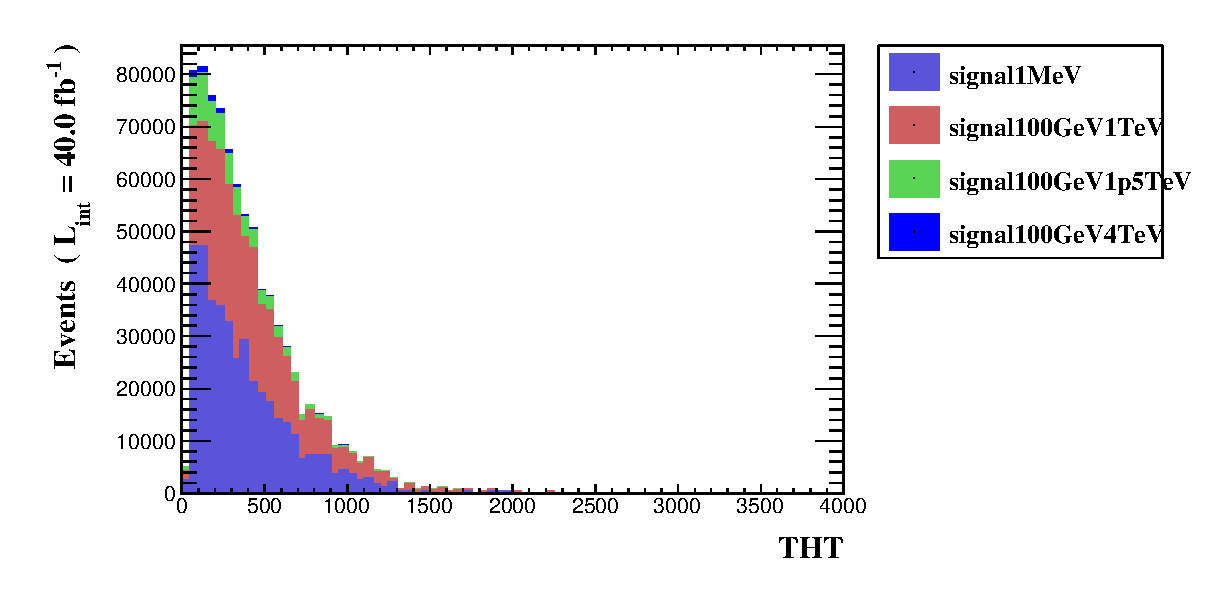
\includegraphics[scale=0.45]{selection_9.eps}\\
\caption{   }
  \end{center}
\end{figure}
      \newpage
\subsection{ Histogram 11}

\textbf{* Plot: MET}\\
   \begin{table}[H]
  \begin{center}
    \begin{tabular}{|m{23.0mm}|m{23.0mm}|m{18.0mm}|m{19.0mm}|m{19.0mm}|m{19.0mm}|m{19.0mm}|}
      \hline
      {\cellcolor{yellow}         Dataset}& {\cellcolor{yellow}         Integral}& {\cellcolor{yellow}         Entries per event}& {\cellcolor{yellow}         Mean}& {\cellcolor{yellow}         RMS}& {\cellcolor{yellow}         \% underflow}& {\cellcolor{yellow}         \% overflow}\\
      \hline
      {\cellcolor{white}         signal1mev}& {\cellcolor{white}         406568}& {\cellcolor{white}         1.0}& {\cellcolor{white}         3.56703e-09}& {\cellcolor{white}         4.096e-09}& {\cellcolor{green}         0.0}& {\cellcolor{green}         0.0}\\
      \hline
      {\cellcolor{white}         signal100gev1tev}& {\cellcolor{white}         340913}& {\cellcolor{white}         1.0}& {\cellcolor{white}         4.36606e-09}& {\cellcolor{white}         5.231e-09}& {\cellcolor{green}         0.0}& {\cellcolor{green}         0.0}\\
      \hline
      {\cellcolor{white}         signal100gev1p5tev}& {\cellcolor{white}         71082}& {\cellcolor{white}         1.0}& {\cellcolor{white}         3.51729e-09}& {\cellcolor{white}         4.485e-09}& {\cellcolor{green}         0.0}& {\cellcolor{green}         0.0}\\
      \hline
      {\cellcolor{white}         signal100gev4tev}& {\cellcolor{white}         7153}& {\cellcolor{white}         1.0}& {\cellcolor{white}         3.04943e-09}& {\cellcolor{white}         3.811e-09}& {\cellcolor{green}         0.0}& {\cellcolor{green}         0.0}\\
\hline
    \end{tabular}
  \end{center}
\end{table}

\begin{figure}[H]
  \begin{center}
    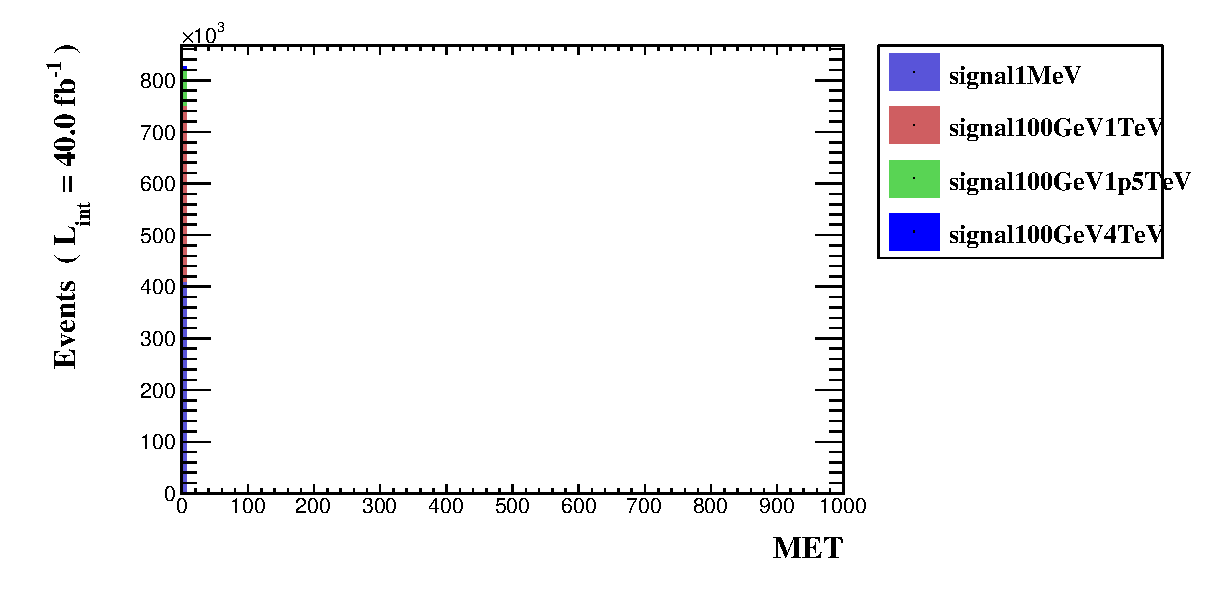
\includegraphics[scale=0.45]{selection_10.eps}\\
\caption{   }
  \end{center}
\end{figure}
      \newpage
\subsection{ Histogram 12}

\textbf{* Plot: TET}\\
   \begin{table}[H]
  \begin{center}
    \begin{tabular}{|m{23.0mm}|m{23.0mm}|m{18.0mm}|m{19.0mm}|m{19.0mm}|m{19.0mm}|m{19.0mm}|}
      \hline
      {\cellcolor{yellow}         Dataset}& {\cellcolor{yellow}         Integral}& {\cellcolor{yellow}         Entries per event}& {\cellcolor{yellow}         Mean}& {\cellcolor{yellow}         RMS}& {\cellcolor{yellow}         \% underflow}& {\cellcolor{yellow}         \% overflow}\\
      \hline
      {\cellcolor{white}         signal1mev}& {\cellcolor{white}         406568}& {\cellcolor{white}         1.0}& {\cellcolor{white}         616.896}& {\cellcolor{white}         471.7}& {\cellcolor{green}         0.0}& {\cellcolor{green}         0.0}\\
      \hline
      {\cellcolor{white}         signal100gev1tev}& {\cellcolor{white}         340913}& {\cellcolor{white}         1.0}& {\cellcolor{white}         745.517}& {\cellcolor{white}         543.9}& {\cellcolor{green}         0.0}& {\cellcolor{green}         0.0}\\
      \hline
      {\cellcolor{white}         signal100gev1p5tev}& {\cellcolor{white}         71082}& {\cellcolor{white}         1.0}& {\cellcolor{white}         580.998}& {\cellcolor{white}         479.7}& {\cellcolor{green}         0.0}& {\cellcolor{green}         0.0}\\
      \hline
      {\cellcolor{white}         signal100gev4tev}& {\cellcolor{white}         7153}& {\cellcolor{white}         1.0}& {\cellcolor{white}         468.042}& {\cellcolor{white}         387.8}& {\cellcolor{green}         0.0}& {\cellcolor{green}         0.0}\\
\hline
    \end{tabular}
  \end{center}
\end{table}

\begin{figure}[H]
  \begin{center}
    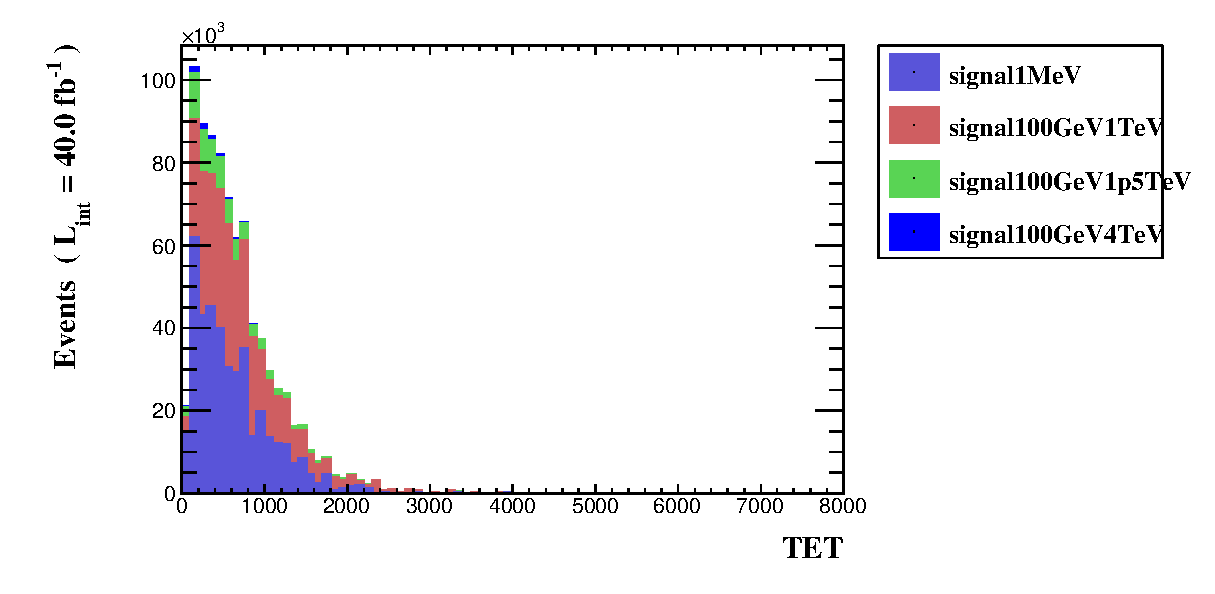
\includegraphics[scale=0.45]{selection_11.eps}\\
\caption{   }
  \end{center}
\end{figure}
      \end{document}
